\chapter{REVIEW OF RELATED LITERATURE}

We will now provide an overview of the \textit{CryptoImg} project, which our study is primarily based on. Then, we define the specific image processing operations we are interested in implementing in this study. Then we will introduce concepts in cryptography and define the four homomorphic cryptosystems we will be testing in the study.

\section{CryptoImg}
A paper published in 2009 by Ziad, et al. attempts to implement privacy-preserving image processing using \textit{CryptoImg}, a library for the Open Source Computer Vision Library (OpenCV)~\cite{bradski_opencv_2000} which implements various homomorphic encryption and image processing routines using the Paillier homomorphic cryptosystem~\cite{ziad_cryptoimg:_2016}. The CryptoImg library assumed a client-server model wherein a client requests image processing operations from a server. A client first encrypts a digital image and sends the image securely to a server, which then operates on the encrypted image without revealing its contents. Then the resulting image is sent back to the client, which decrypts the image to recover the desired output.
\begin{figure*}[!ht]
    \centering
    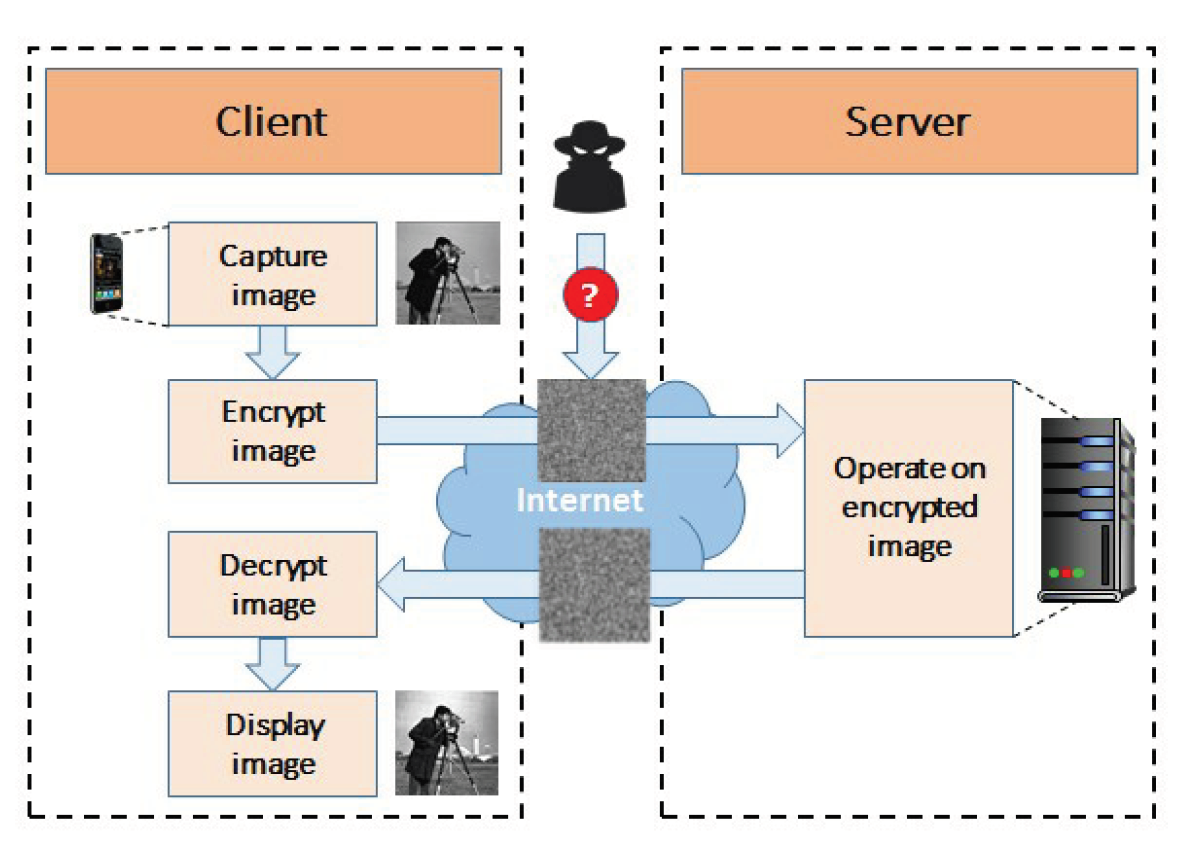
\includegraphics[width=\textwidth,\keepaspectratio]{figures/ClientServerModel.png}
    \caption{Client-server architecture used by \textit{CryptoImg} \cite{ziad_cryptoimg:_2016}}
    \label{fig:clientserver}
\end{figure*}
The \textit{CryptoImg} library implemented the following:
\begin{enumerate}
	\item Extending the Paillier homomorphic cryptosystem which operate on integer plaintexts so that they can operate on real number plaintexts;
	\item Developing protocols for and implementing the following image processing operations
	\begin{enumerate}
		\item Image negation and brightness adjustment
		\item Spatial filters (for noise reduction, edge detection and sharpening)
		\item Morphological operations
		\item Histogram equalization
	\end{enumerate}
\end{enumerate}
For image negation and spatial filters, the protocols specified by \textit{CryptoImg} allow all image processing operations to be performed on the server. However, due to limitations in the Paillier cryptosystem, the protocols presented for morphological operations and histogram equalization require both the client and the server to perform image processing calculations, although the server performs a significant portion of the processing.

Ziad, et al. also showed experimental results establishing the slow performance of image operations under a homomorphic cryptosystem. For instance, while sharpening and applying a Sobel filter each take less than a second when applied to a $512\times 512$ plaintext image, when applied to an encrypted image, sharpening required at least 238.257 seconds, and applying the Sobel filter required at least 147.567 seconds \cite{ziad_cryptoimg:_2016}.

%%limitations = not considering transcendental function evaluation
%%extension to fully homomorphic cryptosystems
%%combined applications in face detection and recognition

We now discuss several limitations in the \textit{CryptoImg} study which we focus on for our research. First, the \textit{CryptoImg} library was limited in the image intensity transformations it implemented. We propose additional protocols to support more computationally intensive intensity transformations.
Second, the \textit{CryptoImg} library only considered the Paillier cryptosystem. We consider testing the performance of other homomorphic cryptosystems, which differ in their processing time and supported operations.

\section{Image Processing Operations}
The \textit{CryptoImg} library implemented several
We discuss two basic types of image processing operations, \textit{intensity transformations}, which map an intensity value to another, and \textit{spatial filters} which consider intensity values from regions of pixels to perform operations such as edge detection, image blurring and sharpening.

We represent a digital image $R$ as an $M \times N$ matrix of pixel intensity values, each value in the range $\left[0, L-1\right]$, for some positive integer $L$. We use $R(x,y)$ represents the entry at the $x$th row and $y$th column of a matrix $R$.

\subsection{Intensity Transformations}
An Intensity transformation on an image $R$ can be defined as a function $T$ which maps a pixel value $r$ to a new value $r^\prime$, which we can write as $r^\prime = T\left(r\right)$. This function is then applied to every pixel in $R$.

The \textit{CryptoImg} library implemented two types of linear intensity transformations: image negation and brightness control.
An image negation transformation is defined as:
\begin{equation}
    T\left(r\right) = L-1-r
\end{equation}
After applying image negation, the resulting image would be similar to a photographic negative~\cite{gonzalez_digital_2008}.

A brightness control transformation with parameter $v$ is defined as:
\begin{equation}
    T\left(r,v\right) = r+v
\end{equation}
The above transformations are linear in terms of the input $r$, and are thus simple to implement under a homomorphic cryptosystem.

In this study we extend the range of intensity transformations to non-linear transformations. Two common non-linear image transformations are the log transformation and power-law transformation~\cite{gonzalez_digital_2008}.

The log transformation is used to enhance dark pixels or increase the dark details of an image by mapping low intensity values to a wider range of values~\cite{gonzalez_digital_2008}. This has the general formula
\begin{equation}
    T\left(r\right) = c \log\left(1 + r\right)
\end{equation}
where $c$ is a constant and $r \ge 0$.

The power-law transformation is a family of transformations that have the form
\begin{equation}
    T\left(r\right) = c r^{\gamma}
\end{equation}
where $c>0$ and $\gamma > 0$.
A power-law transformation defined by the above equation can calibrate the operation of many image capture and output devices such as cameras, printers and displays in a process called \textit{gamma correction}. This ensures reproducibility and accuracy of images being displayed by digital output devices~\cite{gonzalez_digital_2008}.

To implement non-linear intensity transformations using addition and multiplication in a homomorphic system, it is necessary to approximate the logarithm and exponential functions, which may result in higher computational overhead. In our software library implementation, we investigate methods required to approximate the logarithm and functions.

\subsection{Spatial Filtering}
The \textit{CryptoImg} library also implemented \textit{spatial filters}. Spatial filters are operators which determine output pixels using information from neighboring input pixels. To apply a spatial filter to obtain a resulting image $R^\prime$, a convolution is performed between an $m \times n$ matrix $k$, called a kernel, and the original $M\times N$ image $R$.
A convolution between a kernel $k$ and image $R$ which yields a resulting image $R^\prime$, denoted as $R^\prime = k \ast R$, is defined by
\begin{align} \label{eq:spatialfilter}
	R^\prime(x,y) = \sum_{s=1}^m{\sum_{t=1}^n{k(s,t)R(x+s,y+t)}}, \text{ for all } 0\leq x \leq M, 0 \leq y \leq N,
\end{align}

\begin{figure*}[!ht]
    \centering
    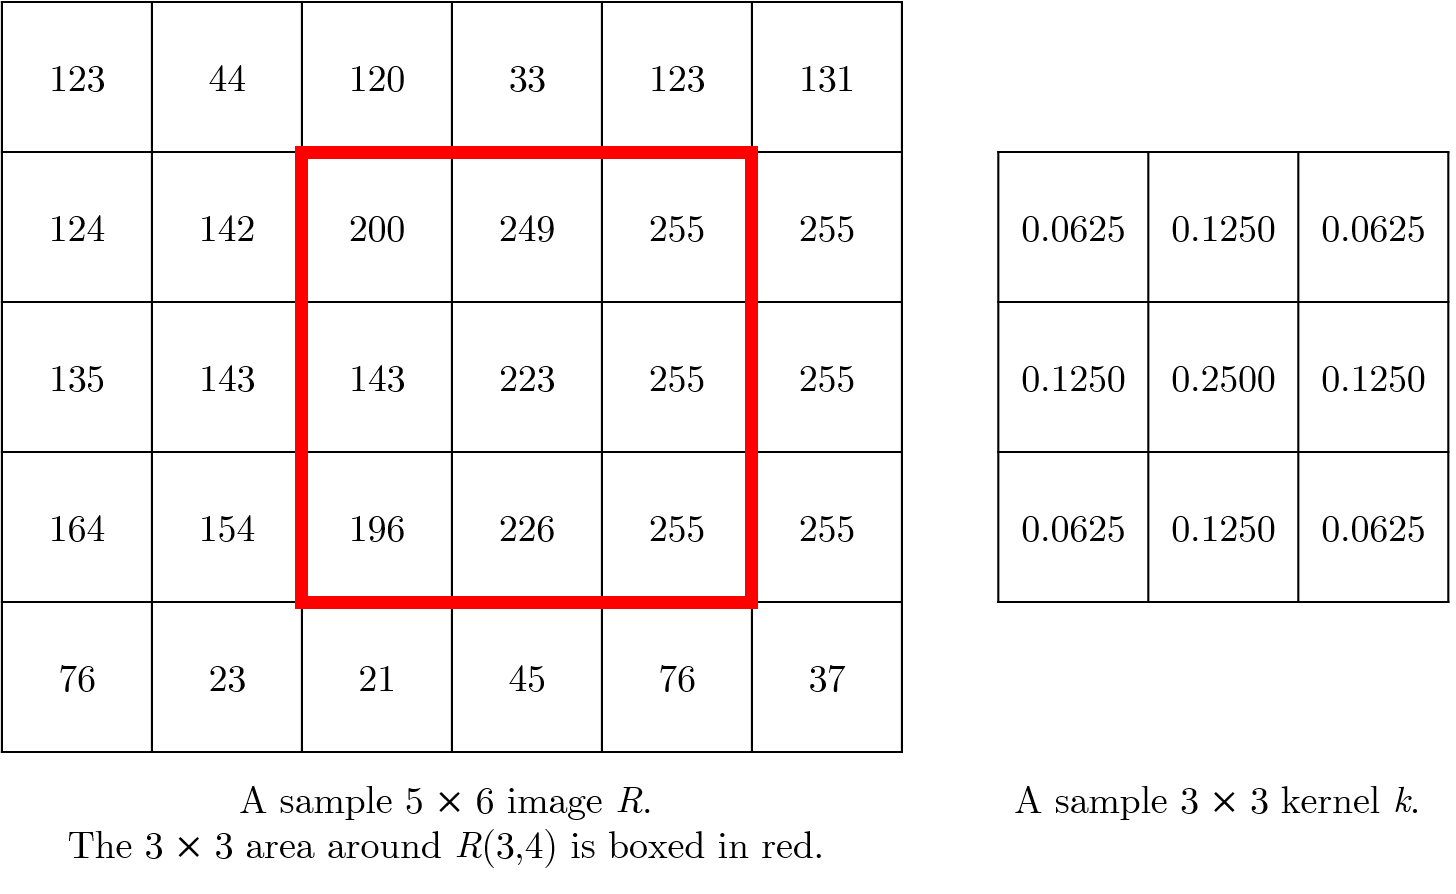
\includegraphics[width=\textwidth,\keepaspectratio]{Figures/SpatialFilter.png}
    \caption{A sample image $R$ and sample kernel $k$.}
    \label{fig:spatialfilter}
\end{figure*}
For example, using the image and $3 \times 3$ kernel given in Figure \ref{fig:spatialfilter}, we can calculate the value in the third row and fourth column of the resulting image $R^\prime$ by adding the products of entries in $k$ with the corresponding entries in $R$, found in an $3 \times 3$ region around $R(3,4)$.
\begin{align*}
	R^\prime(3,4) &= \sum_{s=1}^m{\sum_{t=1}^n{k(s,t)R(3+s,4+t)}}\\
	&= (0.0625\times 200) + (0.1250\times 249) + (0.0625\times 255) \\
	&+ (0.1250\times 143) + (0.2500\times 223) + (0.1250\times 255) \\
	&+ (0.0625\times 196) + (0.1250\times 236) + (0.0625\times 255)\\
	&= 223.
\end{align*}
Since spatial filters take values from a contiguous region of pixels, this presents a difficulty in homomorphic cryptosytems: in order for spatial filters to be performed, the location of each pixel relative to neighboring pixels has to be preserved. This was performed in the implementation of spatial filters in the \textit{CryptoImg} library~\cite{ziad_cryptoimg:_2016}. We wish to implement spatial filters using a similar approach, and assess how preserving spatial correlation between pixels can impact the security of the encrypted image.

\subsection{Common Spatial Filtering Kernels}
Edge detection is used to find and determine the boundaries in an image, commonly used in applications such as image segmentation and feature extraction. This works by detecting so-called \textit{edges}, areas that have abrupt changes in intensity.
One common method of performing edge detection is the Sobel operator, which uses two spatial filters to approximate the gradient of an image. Given an image $R$, and the kernels
\begin{equation}
    g_x =
    \begin{bmatrix}
        -1 & 0 & 1 \\
        -2 & 0 & 2 \\
        -1 & 0 & 1
    \end{bmatrix}
    \qquad\text{and}\qquad
    g_y =
    \begin{bmatrix}
        1 & 2 & 1 \\
        0 & 0 & 0 \\
        -1 & -2 & -1
    \end{bmatrix},
\end{equation}
$g_x \ast R$ yields the horizontal component of the gradient, while $g_y \ast R$ yields the vertical component of the gradient.

There are also spatial filters that perform image smoothing (such as Gaussian blur and box blur, which use the kernels $b_g$ and $b$ respectively in Equation~\ref{eqn:smooth-filters}) and image sharpening~\cite{gonzalez_digital_2008}.
\begin{equation}
    \label{eqn:smooth-filters}
    b_g = \frac{1}{16}
    \begin{bmatrix}
        1 & 2 & 1 \\
        2 & 4 & 2 \\
        1 & 2 & 1
    \end{bmatrix}
    \qquad
    b = \frac{1}{9}
    \begin{bmatrix}
        1 & 1 & 1 \\
        1 & 1 & 1 \\
        1 & 1 & 1
    \end{bmatrix}
\end{equation}

%% TODO: specific list of kernels to use for this study

%facial recognition - theory
\section{Facial Detection and Recognition}
%% TODO: Brian dump ur stuff here

Since simple image operations an be done within a homomorphic cryptosystem, these operations can be assembled together in order to do more complex operations. A prominent application of image processing that often uses complex image operations is \textit{facial recognition}.

Traditional facial recognition algorithms rely on detecting salient features in a face image. One of the popular facial recognition algorithms is \textit{eigenfaces}.
% Traditional facial recognition algorithms rely on detecting salient features in a face image. Two of the popular facial recognition algorithms are \textit{eigenfaces} and \textit{Haar cascades}.

\subsection{Eigenfaces}

Proposed by Matthew Turk and Alex Pentland, the eigenfaces method uses principal component analysis (PCA) in order to express an input image as a linear combination of eigenfaces \cite{turk_eigenfaces_1991}. An \textit{eigenface} is a principal component, or more simply an eigenvector that represents a certain variation between the face images which are taken from the initial training set. The number of resulting eigenfaces is equal to the number of face images in the training set.

In the enrollment process, $M$ face images $\Theta_1, \ldots, \Theta_M$, each of size $p \times q$, are taken in to comprise the initial training set. The training images can be represented as vectors of length $N = pq$, where each row of an image is concatenated together.

The average of the training images, denoted as $\Psi$, is 
\[ \Psi = \frac{1}{M} \sum_{i=1}^{M} \Theta_i \]

The \textit{difference vectors} are then computed as $\Phi_i = \Theta_i - \Psi$. PCA is applied on the covariance matrix of the vectors
\[ \mathbf{C} = \frac{1}{M} \sum_{i=1}^M \Phi_i \Phi_i^\top = \frac{1}{M} \mathbf{A}\mathbf{A}^\top,\]
where $\mathbf{A}$ is an $N \times M$ matrix defined by $\left[\Theta_1 \quad \Theta_2 \quad \cdots \quad \Theta_M\right]$, in order to determine the orthonormal eigenvectors \cite{hutchison_privacy-preserving_2009}.

Directly computing the covariance matrix and then applying PCA will become inefficient for large sizes of $\mathbf{A}$, since computing for $\mathbf{A}\mathbf{A}^\top$ results in an $N \times N$ matrix, which can get drastically large because it is dependent on the size of the image. On the other hand, computing for $\mathbf{A}^\top\mathbf{A}$ only results in an $M \times M$ matrix, which is much smaller than the previous one because it is just dependent on the number of face images in the training set. Now, we can apply PCA to $\mathbf{A}^\top\mathbf{A}$ along with some post-processing to obtain the eigenvectors \cite{hutchison_privacy-preserving_2009}. 

Instead of getting the eigendecomposition of the covariance matrix by explicitly computing the eigenvalues and eigenvectors of $\mathbf{C}$, we can also apply \textit{singular value decomposition} (SVD) on the matrix $\Phi^\top$. This is because SVD works through a divide-and-conquer method which results in greater numerical stability, while eigendecomposition simply uses the traditional QR factorization \cite{nakatsukasa_stable_2013, gu_divide-and-conquer_1995}. Upon applying SVD, we now get the eigenvectors $\mathbf{u}_1, \ldots, \mathbf{u}_M$ and their corresponding eigenvalues $\lambda_1, \ldots, \lambda_M$.

We choose $K$ eigenvectors $\mathbf{u}_1, \ldots, \mathbf{u}_K$ such that it comprises a set associated with the $K$ largest eigenvalues, where $K$ is much smaller than $M$. This set is now the \textit{face space}. Then, the images $\Theta_1, \ldots, \Theta_K$ are projected onto the face space spanned by the eigenfaces to determine the weight vectors $\Omega_1, \ldots, \Omega_K$.

To perform the recognition process, the algorithm projects the input image $\Gamma$ onto the face space, and then comparing the projected image $\bar{\Omega} = \mathbf{u}_i\left(\Gamma - \Psi\right)$ with each eigenface in the face space using a metric such as the Euclidean distance. Thus it is computed as $d_i = \left\lVert \Omega_i -\bar{\Omega} \right\rVert$ for all $i=1,\ldots,K$, where $\left\lVert \cdot \right\rVert$ denotes the Euclidean norm.

Then, a match can be reported if the smallest possible distance is smaller than the given threshold value $T$. 
\newcommand{\argmin}{\mathop{\mathrm{arg\,min}}}  
\[\text{ID} = \begin{cases}\argmin_i d_i & \text{if } \min_i d_i \le T \\\emptyset & \text {otherwise}\end{cases}
\]

% \subsection{Haar Cascades}
% A \textit{Haar cascade classifier} is another method for facial recognition by Paul Viola and Michael Jones \cite{viola_robust_2004}. It uses Haar-like features to detect regularities in a face image. A \textit{Haar-like feature} looks at a certain rectangular region of the image through a filter-like window.

% \begin{figure}[!h]
%     \centering
%     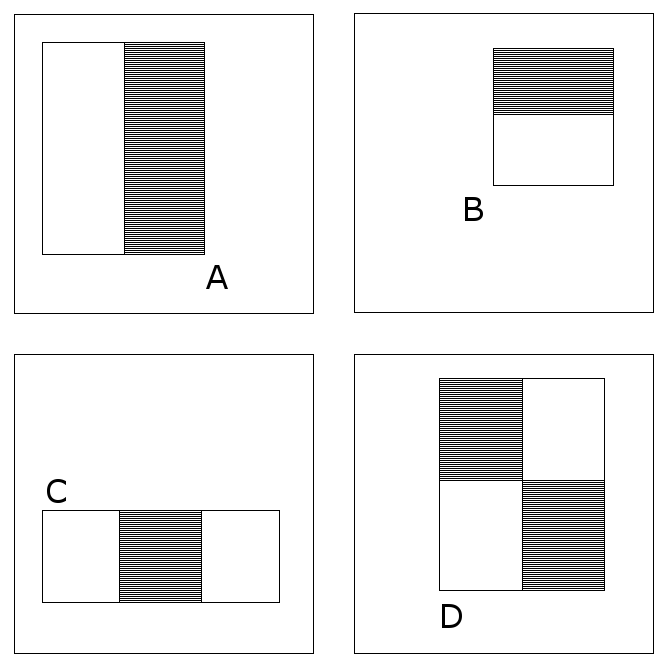
\includegraphics[width=7cm]{figures/haarfeatures2.png}
%     \caption{Examples of Haar-like features \cite{viola_robust_2004}.}
% \end{figure}

% A Haar-like feature is composed of black and white rectangles, and arranged such that it detects a presence or an absence of a particular image feature or regularity of interest. For example, a feature may detect the difference in intensities between the eyes and the cheeks, another feature would detect the edges of the face, and another one would detect depending on the location of the eyes. The detection is done by summing up the intensities within the black region and the white region, and then calculating the difference.

% Getting the sum of pixel intensities within a region na\"{i}vely would become inefficient as the size of the rectangular region increases, so a data structure called an \textit{integral image} is used to allow more efficient detection of Haar-like features. In other words, an integral image is essentially a two-dimensional range sum that can compute sums of rectangular regions in constant time, regardless of the size of the regions.

% Most of the Haar-like features are irrelevant, because a feature that works in a certain part of the image would not necessarily work in another part. The whole process may become needlessly inefficient due to computational time being potentially wasted on a huge number of irrelevant features, even though computing for a feature is said to be efficient. That is why we need to select the best features and use those to form a strong classifier in a process called AdaBoost \cite{viola_robust_2004}.

% In itself, a Haar-like feature is considered as a \textit{weak classifier}, the probability of detecting a certain feature is slightly greater than detecting at random \cite{viola_robust_2004}. So a large number of Haar-like features must be used together by forming them into cascade classifiers in order to achieve a sufficient enough accuracy. The resulting strong classifier would then be a linear combination of the weak classifiers.

% Each stage in the cascade classifier consists of weak classifiers that uses decision stumps, so that the weak classifiers can classify many examples correctly. A \textit{decision stump} can be defined as
% \[h \left(x, f, p, \theta \right) = \begin{cases}1 & \text{if } pf(x) < p\theta\\ 0 & \text{otherwise}\end{cases}
% \]
% where $x$ is a fixed window of the image, $f$ is the feature, $p$ is the polarity, and $\theta$ is the threshold \cite{viola_robust_2004}.

% Each stage also labels the region as positive (meaning that there is a face within the region), and negative (if none). If the detector sees the region as negative, it is immediately discarded and not processed anymore. Otherwise if the region is labeled as positive, it moves to the next stage for further processing. When a region successfully completes all the stages, it can be considered as a face region.

\section{Homomorphic Cryptosystems}

A cryptosystem~\cite{bauer_cryptosystem_2005} consists of an encryption function $\mathcal{E}$ and a decryption function $\mathcal{D}$, which operate on plaintexts, ciphertexts and keys. A \textit{plaintext} is text that can be commonly understood within a larger group. Given a \textit{key}, the encryption function maps a plaintext to some \textit{ciphertext}, which can only be understood by authorized parties. The decryption function similarly maps a ciphertext back to its corresponding plaintext, given an appropriate key. By sending data as ciphertext and only exposing the corresponding plaintexts to authorized parties who have access to the appropriate keys, secure data transmission can be achieved.

Cryptosystems may be classified as either \textit{symmetric} or \textit{asymmetric}. 
In symmetric-key cryptosystems, the same key is used for both encryption and decryption. As a consequence, symmetric-key cryptosystems must be implemented with a secure key exchange protocol, so that both the sender and receiver have access to the same key while keeping the key secret. 
Prominent examples of symmetric-key cryptosystems are the Data Encryption Standard (DES), and its replacement, the Advanced Encryption Standard (AES).

On the other hand, asymmetric-key (or public-key) cryptosystems use separate keys for encryption and decryption. The encryption key (also called the \textit{public key}) is shared publicly, while the decryption key (also called the \textit{private key}) is kept secret. Since the public key and private keys differ, secure key exchange protocols are not required. The security of asymmetric-key cryptosystems rely on the intractability of certain computational problems, for example, the RSA cryptosystem depends on the difficulty of big integer factorization~\cite{rivest_method_1978}, while the ElGamal cryptosystem depends on the difficulty of the discrete logarithm problem~\cite{blakley_public_1985}.

Homomorphic cryptosystems are a special type of cryptosystem which allows operations to be performed on recovered plaintexts by performing corresponding operations on ciphertexts. This allows for secure computation in the plaintext space $\mathcal{P}$, the set of all plaintexts, by performing operations in the ciphertext space $\mathcal{C}$, the set of all ciphertexts. 

Suppose that in a public-key cryptosystem, $\mathcal{E}_k \left(p \right)$ is the encryption function which uses a public key $k$, and $\mathcal{D}_l \left(c \right)$ is the decryption function which uses a private key $l$. The cryptosystem is said to be homomorphic if its encryption function is homomorphic, that is, if it satisfies the relation
\begin{equation}
    \label{eq:homomorphic_definition_encryption}
    \mathcal{E}_k \left(p_1 \boxplus p_2\right) = \mathcal{E}_k \left(p_1\right) \boxdot \mathcal{E}_k \left(p_2\right)
\end{equation}
where $p_1, p_2 \in \mathcal{P}$ are plaintexts, and $\boxplus$ and $\boxdot$ are operations in $\mathcal{P}$ and $\mathcal{C}$ respectively~\cite{fontaine_survey_2007}. By applying the decryption function $\mathcal{D}_l$ to both sides of equation~\ref{eq:homomorphic_definition_encryption}, we see that a homomorphic cryptosystem also satisfies~\cite{li_elliptic_2012}
\begin{equation}
    \label{eq:homomorphic_definition_decryption}
    p_1 \boxplus p_2 = \mathcal{D}_l \left( \mathcal{E}_k \left(p_1\right) \boxdot \mathcal{E}_k \left(p_2\right) \right).
\end{equation}
In other words, a homomorphic cryptosystem allows operations to be performed on recovered plaintexts by performing corresponding operations on ciphertexts. Using a homomorphic cryptosystem, secure computation can be achieved by encrypting plaintexts and then operating on the ciphertexts. We note that the operations $\boxplus$ and $\boxdot$ need not be the same. A simple operation in the plaintext space may require a computationally intensive operation in the ciphertext space.

Homomorphic cryptosystems can be classified according to the supported plaintext operation(s) $\boxplus$ which can be securely computed. The cryptosystem is said to be \textit{additively homomorphic} if the plaintext operation $\boxplus$ is addition, and the cryptosystem is said to be \textit{multiplicatively homomorphic} if the plaintext operation $\boxplus$ is multiplication. Homomorphic cryptosystems which only allow for a limited set of operations to be computed securely are called \textit{partially homomorphic} while those which allow for arbitrary operations to be computed securely are called \textit{fully homomorphic}. Numerous partially homomorphic and fully homomorphic cryptosystems have been developed in the literature. This study compares several of them, which we will now introduce in detail. 


%Homomorphic cryptosystems
%Some examples of homomorphic cryptosystems include the Goldwasser--Micali cryptosystem~\cite{goldwasser_probabilistic_1984} and the Paillier cryptosystem~\cite{stern_public-key_1999}. Even some classic public-key cryptosystems are homomorphic, both RSA and ElGamal are multiplicatively homomorphic, while elliptic curve cryptosystems are additively homomorphic~\cite{li_elliptic_2012}. These cryptosystems, while relatively efficient, only support a limited set of operations on the encrypted data.

%However, there exists \textit{fully homomorphic} cryptosystems, which are not limited to a fixed set of operations, but allow any arbitrary operations on the ciphertext. The first  fully homomorphic cryptosystem was presented by Gentry in 2009. Gentry's cryptosystem, which uses lattice-based cryptography, allows the computation of computation of arbitrary Boolean circuits on binary data~\cite{gentry_fully_2009, shortell_secure_2016}. New algorithms based on Gentry's initial ideas have since been made~\cite{ sen_homomorphic_2013}. One notable example is fully homomorphic cryptosystem by Smart and Vercauteren,~\cite{hutchison_fully_2010}, later improved by Gentry and Halevi ~\cite{hutchison_implementing_2011} which relies on cyclotomic number fields. In 2016, Dasgupta and Pal proposed a fully homomorphic cryptosystem based on polynomial rings~\cite{dasgupta_design_2016}. These two cryptosystems are examples of fully homomorphic cryptosystems which have significantly simpler encryption, decryption, addition and multiplication algorithms.

\section{Partially Homomorphic Cryptosystems}

In this section, we will present two classical partially homomorphic cryptosystems (PHEs) which we will be testing in the study: the Paillier cryptosystem and the DGK cryptosystem. Both of these cryptosystems encrypt integer plaintexts and are additively homomorphic and allow for the multiplication of a plaintext scalar. We will then show how these PHEs may be adapted for secure floating-point computation. 

\subsection{The Paillier Cryptosystem}
The Paillier cryptosystem \cite{stern_public-key_1999}, developed by Pascal Paillier, is a probabilistic encryption scheme which is based on the composite residuosity class problem.

\subsubsection{Key Generation}
We choose two large primes $p$ and $q$, and set $n = pq $ and $ \lambda = \mathrm{lcm}\left(p-1,q-1\right)$.
We then define $L\left(x\right)$ to be the largest integer $v$ greater than zero such that $x-1 \geq vn$.
Then we select an integer $g$ such that $\gcd\left(L\left(g^\lambda \bmod n^2\right), n\right) = 1$ and $0\leq g \leq n^2$.
We define the public key as $(g,n)$ and the private key as $(p,q)$.

\subsubsection{Encryption and Decryption}
The encryption function to encrypt a plaintext $m \in \mathbb{Z}_n$ given a public key $(g,n)$ is defined as
\begin{align*}
  E(m) = g^m \cdot r^n \mod{n^2},
\end{align*}
where $r$ is a random non-negative integer less than $n^2$.

The decryption function to decrypt a ciphertext $c \in \mathbb{Z}_{n^2}$ given a private key $(p,q)$ is defined as:
\begin{align*}
  D(c) = L(c^\lambda \bmod n^2) \times (L(g^\lambda \bmod n^2))^{-1} \mod n
\end{align*}

\subsubsection{Homomorphic Properties of the Paillier Cryptosystem}
The Paillier cryptosystem supports additive homomorphism as well as the multiplication of a plaintext scalar to an encrypted message. These operations are defined as follows.
For all $m_1,m_2 \in \mathbb{Z}_n$ and $k\in \mathbb{N}$, the following homomorphic properties hold.
\begin{align*}
  D(E(m_1)g^k\bmod n^2)=(m_1+k)\bmod n & \text{ (add a plaintext constant)}\\
  D(E(m_1)E(m_2)\bmod n^2)=(m_1+m_2)\bmod n & \text{ (ciphertext addition)}\\
  D(E(m_1)^k\bmod n^2)= km_1\bmod n & \text{ (multiply a plaintext constant)}
\end{align*}

\subsection{The DGK Cryptosystem}
The DGK cryptosystem was published by Damg{\aa}rd, Geisler, and Kr{\o}igaard in 2007 in an effort to create a secure integer comparison scheme \cite{pieprzyk_efficient_2007, cryptoeprint:2008:321} which is widely used in the literature \cite{veugen_improving_2012}.

\subsubsection{Key Generation}
We denote $k,t,\ell$ as security parameters of the scheme, where $k>t>\ell$.
Let $p,q$ be primes such that
we can choose two $t$-bit primes $v_p$ and $v_q$ such that $v_p | (p-1)$ and $v_q | (q-1)$, and a small prime $u$ such that $u | (p-1)$ and $u | (q-1)$.
We denote $n = pq$.
We choose $g$ to be an integer of order $uv_pv_q$ and $h$ to be of order $v_pv_q$.

The DGK cryptosystem encrypts plaintexts in $\mathbb{Z}_u$ to ciphertexts in $\mathbb{Z}_n^\ast$.

The public key is $(n,g,h,u)$ and the private key is $(p,q,v_p,v_q)$.

\subsubsection{Encryption and Decryption}
To encrypt a message $m \in \mathbb{Z}_u$, the encryption function is defined as:
\begin{align*}
  E(m) = g^m \cdot h^r \mod{n},
\end{align*}
where $r$ is a random integer in $\mathbb{Z}_n$ which is longer than $2t$ bits.

To decrypt a ciphertext $c \in \mathbb{Z}_n^\ast$, decryption is achieved by first computing $c^{v_pv_q}$.
\begin{align*}
	c^{v_pv_q} \bmod n
	&= (g^m \cdot h^r)^{v_pv_q} \bmod n\\
	&= (g^{v_pv_q})^m \bmod n
\end{align*}
Since $(g^{v_pv_q})^m$ has order $u$, there is a one-to-one correspondence between plaintexts in $\mathbb{Z}_u$ and  $(g^{v_pv_q})^m$. A lookup table can thus be generated privately to successfully recover $m$.

\subsubsection{Homomorphic Properties of the DGK Cryptosystem}
The DGK cryptosystem supports additive homomorphism as well as the multiplication of a plaintext scalar to an encrypted message. These operations are defined as follows.
For all $m_1,m_2 \in \mathbb{Z}_u$ and $k\in \mathbb{N}$, the following homomorphic properties hold.
\begin{align*}
    D(E(m_1)g^k)=(m_1+k)\bmod u & \text{ (add a plaintext constant)}\\
    D(E(m_1)E(m_2))=(m_1+m_2)\bmod u & \text{ (ciphertext addition)}\\
    D(E(m_1)^k)= km_1\bmod u & \text{ (multiply a plaintext constant)}
\end{align*}

As the multiplicative homomorphism was not presented in the original paper, we provide a short proof here.
\begin{proof}
  Let $m \in \mathbb{Z}_u$ and $k\in \mathbb{N}$.
  We consider $E(m)^k = (g^m \cdot h^r \bmod{n})^k\bmod n$.
  \begin{align*}
    (g^m \cdot h^r \bmod{n})^k \bmod n
    &= (g^m \cdot h^r)^k \bmod{n}\\
    &= (g^m)^k \cdot (h^r)^k \bmod{n}\\
    &= g^{km} \cdot (h^{kr}) \bmod{n}
  \end{align*}
  Since $r$ is a random integer, $kr$ is also a random integer, Therefore, $g^{km} \cdot (h^{kr}) \bmod{n} = D(E(m)^k)$ is a valid encryption of the message $km$.
\end{proof}

\subsection{Floating-Point Arithmetic using PHEs}
\label{sec:fp_arithmetic}
We have discussed the Paillier and DGK cryptosystems, which encrypt and allow similar operations on encrypted integers. We will now show how these PHEs may be extended to a system which allows for secure floating-point computation.

In this section, we let $\oplus$ and $\otimes$ represent the homomorphic operations which correspond to the addition and multiplication of integers in a PHE, respectively. 

\subsubsection{Extension to Floating-Point Numbers}
\label{sec:fp_operations}
We can use the following protocol described in~\cite{ziad_cryptoimg:_2016} in order to extend Paillier and DGK to floating-point numbers.

We represent a floating-point (FP) number as a pair of two integers $(m,e)$ representing the mantissa and exponent of the FP number with respect to a base $b$. The mantissa $m$ is encrypted, while the exponent $e$ is unencrypted.
Let $a,b,c$ be FP numbers represented by the pairs $(m_a,e_a),(m_b,e_b),(m_c,e_c)$ respectively. We define the corresponding FP number operations as follows:
\begin{description}
  \item[Addition.]
    To compute $E\left(c\right)=E\left(a+b\right)$ we compute
	\begin{align*}
		E\left(m_c\right) &= 
		\begin{cases}
			E\left(m_a\right) \oplus \left(b^{e_b-e_a} \otimes E\left(m_b\right)\right) & \text{if } e_a \leq e_b \\
			E\left(m_b\right) \oplus \left(b^{e_a-e_b} \otimes E\left(m_a\right)\right) & \text{if } e_a > e_b
		\end{cases}, \\
		e_c &= 
		\begin{cases}
			e_a & \text{if } e_a \leq e_b \\
			e_b & \text{if } e_a > e_b
		\end{cases}.
	\end{align*}
  \item[Scalar multiplication.]
    To compute $E\left(c\right) = E\left(ab\right)$, where $a$ and $E\left(b\right)$ are known (i.e., $m_a$ is not encrypted), we compute
    \begin{align*}
      E\left(m_c\right) &= m_a \otimes E\left(m_b\right),\\
      e_c &= e_a + e_b.
    \end{align*}
\end{description}

\subsubsection{Secure Division}
We can use the following two-party scheme defined in~\cite{boukoros_lightweight_2017} to perform privacy-preserving division.

Suppose Bob has $E\left(x\right)$ and $E\left(y\right)$ and wants to obtain $E\left(x/y\right)$ without exposing the value of either variable.
\begin{itemize}
	\item Bob first selects a random non-zero number $r$ and computes $E\left(rx\right)$ and $E\left(ry\right)$. Bob can do this since $r$ is a plaintext constant.
	\item Bob sends $E\left(rx\right)$ and $E\left(ry\right)$ to Alice, who decrypts both values and computes $x/y$ in the plaintext domain.
	\item Alice encrypts and sends $E\left(x/y\right)$ to Bob.
\end{itemize}

\subsubsection{Secure Exponentiation}
\label{ssec:exponentiationprotocol}
 We can use the following two-party scheme, adapted from the protocol to calculate Euclidean distances used in \cite{hutchison_privacy-preserving_2009}, in order to perform secure exponentiation.

Suppose Alice encrypts an integer $x$ and sends it so Bob has $E\left(x\right)$, and wants to obtain $E\left(x^2\right)$ without exposing the value of $x$.
\begin{itemize}
	\item Bob first selects a random integer $r$ and computes $E\left(x+r\right)$. Bob can do this since $r$ is a plaintext constant.
	\item Bob sends $E\left(x+r\right)$ to Alice, who decrypts the ciphertext to obtain $x+r$.
	\item Alice squares $x+r$ and encrypts the result. She sends $E\left(\left(x+r\right)^2\right)$ to Bob.
	\item Bob computes $E\left(-2rx + r^2\right)$. He then computes
	\begin{align*}
		E\left(\left(x+r\right)^2\right)E\left(-2rx + r^2\right) = E\left(x^2\right).
	\end{align*}
\end{itemize}

\subsubsection{Secure Multiplication}
We can use the secure squaring protocol to arrive at a secure multiplication protocol, which then allows for the evaluation of polynomials.
Suppose Alice encrypts integers $x$ and $y$, and Bob has $E\left(x\right), E\left(y\right)$ and wants to obtain $E\left(xy\right)$.
\begin{itemize}
	\item Bob acquires $E\left(x^2\right)$ and $E\left(y^2\right)$ using the secure squaring protocol.
	\item Bob sends $E\left(x+y\right)$ to Alice, who decrypts the ciphertext to obtain $x+y$.
	\item Alice sends $E\left(\left(x+y\right)^2\right)$ to Bob.
	\item Bob then computes
	\begin{align*}
		\frac{1}{2}E\left(\left(x+y\right)^2\right)E\left(x^2\right)^{-1}E\left(y^2\right)^{-1} &= \frac{1}{2}E\left(\left(x+y\right)^2 - x^2 - y^2\right)\\
		&= \frac{1}{2}E\left(2xy\right)\\
		&= E\left(xy\right).
	\end{align*}
\end{itemize}

By applying these extensions to the Paillier and DGK cryptosystems, privacy-preserving floating-point arithmetic can be acheived. 

\section{Fully Homomorphic Cryptosystems}

We will also be testing fully homomorphic cryptosytems, which allow aribitrary computation on encrypted data.
While generally being more flexible, fully homomorphic cryptosytems are known to be significantly slower than partially homomorphic cryptosytems; improving the efficiency of fully homomorphic cryptosytems is an active area of research \cite{sen_homomorphic_2013}.

We will present two such cryptosystems, the Dasgupta--Pal cryptosystem, which we present in full to explain a correction we propose to it, and the BGV cryptosystem, which has open source implementations availble primarily used in homomorphic cryptography research.

\subsection{The Dasgupta--Pal Cryptosystem}
The Dasgupta--Pal cryptosystem is a fully homomorphic cryptosystem proposed in 2016 by Smaranika Dasgupta and S. K. Pal \cite{dasgupta_design_2016}, which encrypts integer plaintexts in $\mathbb{Z}_n$ to polynomial ciphertexts. We begin our presentation of the Dasgupta--Pal cryptosystem with the following definition.

Given a message $m \in \mathbb{Z}$, we denote
\begin{align*}
		m_p(x) = a_0 + a_1x + a_2x^2 + \cdots + a_kx^k
\end{align*}
where $a_ka_{k-1}\cdots a_2a_1_0$ is the binary representation of $m$.

In the original scheme presented in \cite{dasgupta_design_2016}, the secret key $S_k$ is set to be a large prime. In Appendix \ref{chap:correction}, we present a case where the Dasgupta--Pal cryptosystem fails and prove that setting the secret key $S_k = 2p$, where $p$ is a large prime, corrects errors in the Dasgupta--Pal cryptosystem.
We now decribe the correct cryptosystem.
\subsubsection{Corrected Dasgupta--Pal Cryptosystem Description}
Let $\ell$ denote the security parameter of the cryptosystem.
Let $S_k = 2p$, where $p$ is a prime number with $\ell - 1$ bits.
Choose a random even integer $z$ of length $\log_2{\ell}$.

Let the secret key be $S_k$, and let the refresh key be $R_k = z \cdot S_k$. The secret key is kept private to the encrypting/decrypting parties, while the refresh key is made publicly available.

The scheme defines the encryption algorithm for a message $m$ as follows:
\begin{align*}
	E(m) = y(x) + S_k\times d(x)
\end{align*}
where
$y(x)$ is a polynomial of degree $n$ such that $m_p(x) \equiv y(x) \bmod S_k$ and $d(x)$ is a randomly chosen polynomial of degree $n$. This encrypts each coefficient of of $m_p(x)$ by adding some multiple of $S_k$ to it. Through this process, each bit of the message is encrypted separately.

Furthermore, the decryption algorithm to recover $m_p(x)$ from a ciphertext polynomial $c(x)$ as
\begin{align*}
	m_p(x) = c(x) \bmod S_k \bmod 2.
\end{align*}
Thus $D(c(x))$ is defined as the integer recovered from the coefficients of the polynomial $c(x) \bmod S_k \bmod 2$.

Dasgupta and Pal note that homomorphic operations on ciphertext introduce noise which may interfere with decryption, due to the potential increase in ciphertext values.
To eliminate noise from a polynomial ciphertext, the following refresh function is used:
\begin{align*}
	R(c(x)) = c(x) \bmod R_k.
\end{align*}

\subsubsection{Homomorphic Properties of the Dasgupta--Pal Cryptosystem}
It has been shown \cite{dasgupta_design_2016} that the following properties hold for all integer messages $m_1, m_2 \in \mathbb{Z}_n$ in the Dasgupta--Pal cryptosystem. These properties arise since each coefficient in a ciphertext polynomial is essentially an independently encrypted bit of the original message.
\begin{description}
	\item[XOR on ciphertexts]
	A bitwise exclusive or (XOR) operation on integer messages can be achieved by adding the coefficients pairwise between two ciphertexts.
	\begin{align*}
		D(E(m_1)+E(m_2)) = m_1 \text{ XOR } m_2
	\end{align*}
	\item[AND on ciphertexts]
	Similarly, pair-wise multiplication corresponds to bitwise AND of integer messages.
	\begin{align*}
		D(E(a) \otimes E(b)) = a \text{ AND } b = ab \bmod 2
	\end{align*}
	where $\otimes$ denotes pairwise multiplication,
	\begin{align*}
		\sum_{i=1}^n{a_ix^i} \otimes \sum_{i=1}^n{b_ix^i} = \sum_{i=1}^n{a_ib_ix^i}.
	\end{align*}
\end{description}

Arbitrary computation on data can thus be achived using these bitwise operations. While the Dasgupta--Pal cryptosystem requires significant amounts of memory, as each bit of plaintext is encrypted into an integer, this approach provides a flexible method to perform relatively fast arbitrary computation on encrypted data. Encryption and decryption in the Dasgupta--Pal cryptosystem are accomplished using few arithmetic operations.

\subsection{HElib and the BGV Cryptosystem}
The BGV (Brakerski--Gentry--Vaikuntanathan) cryptosystem \cite{cryptoeprint:2011:277} is a fully homomorphic cryptosystem created based on the ring-learning with error problem. The BGV cryptosystem was constructed to surpass the limitations of prior fully homomorphic cryptosystems, which were based on the first fully homomorphic cryptosystem by Gentry \cite{gentry_fully_2009}.

The details regarding the construction of the BGV cryptosystem are beyond the scope of this paper. For this study, we will be using \textit{HElib} \cite{garay_algorithms_2014}, an open-source library which implements the BGV cryptosystem with optimizations to improve efficiency. Evaluation of operations on 120 inputs in HELib was performed in around 4 minutes, with an average of 2 seconds to process a single input \cite{hutchison_fully_2010,cryptoeprint:2011:566}.

The \textit{HElib} library has been adapted to Python using the Pyfhel library \cite{pyfhel_2018} maintained by Ibarrondo, Laurent (SAP) and Onen (EURECOM), and licensed under the GNU GPL v3 license. The Pyfhel library is a Python API for the HElib library, which supports the following operations on vectors/scalars of integers or binary ciphertexts:
\begin{itemize}
	\item Arithmetic operations: addition, subtraction, multiplication;
	\item Binary operations: AND, OR, NOT, XOR.
\end{itemize}

%facial recognition - implementation
\section{Related Work and Previous Implementations}

%% THIS SECTION IS MARKED FOR DELETION / AMPUTATION
% CryptoImg

% example of homomorphic encryption / image manipulation past work

% minor limitation: improvement on previous work, but not a direct comparison

% major limitation: does not discuss security: are modified images also secure?

There has been work done regarding the application of homomorphic cryptosystems in image processing. In particular, Ziad, et al. introduced a library called \textit{CryptoImg} that uses the homomorphic properties of the Paillier cryptosystem to apply image operations securely \cite{ziad_cryptoimg:_2016}. This shows that it is indeed possible to do various image operations in a homomorphic cryptosystem. Ziad, et al. also showed experimental results establishing the slow performance of image operations uner a homomorphic cryptosystem. For instance, while sharpening and applying a Sobel filter each take less than a second when applied to a $512\times 512$ plaintext image, when applied to an encrypted image, sharpening required at least 238.257 seconds, and applying the Sobel filter required at least 147.567 seconds \cite{ziad_cryptoimg:_2016}.

However, a major limitation of \textit{CryptoImg} is that it does not consider image security. Even though the authors have established that the Paillier cryptosystem itself cannot be broken \cite{ziad_cryptoimg:_2016}, we believe that a cryptanalysis of the encrypted images after they have been operated is necessary, since image operations may be considered additional information in a known plaintext attack.

Furthermore, Ziad, et al. only presented a visual comparison and evaluation to establish the quality of the recovered images. We believe that additional image quality benchmarks, such as those presented in \cite{ahmed_benchmark_2016, ahmad_efficiency_2012}, would allow for quantitative comparisons of image quality.

This study can be further improved by also considering the use of fully homomorphic cryptosystems such as the one presented by Dasgupta and Pal \cite{dasgupta_design_2016}, and the fully homomorphic cryptosystem introduced by Smart and Vercauteren \cite{hutchison_fully_2010} and improved by Gentry and Halevi  \cite{hutchison_implementing_2011}. These fully homomorphic cryptosystems have yet to be implemented for image processing operations.

% HElib
Another related work would be the implementation of a fully homomorphic encryption. Halevi and Shoup \cite{garay_algorithms_2014} introduced \textit{HElib}, a library that implements the Brakerski--Gentry--Vaikuntanathan (BGV) homomorphic cryptosystem. This library also makes use of various optimizations to speed up the homomorphic operations, due to homomorphic cryptosystems being slower than other cryptosystems \cite{sen_homomorphic_2013}.


\section{Summary}
We have seen how privacy-preserving image operations have been implemented in the literature using partially homomorphic cryptosystems. \textit{CryptoImg} provided a suite of linear image processing operations using the Paillier cryptosystem, while Erkin, et al. have implemented a privacy-preserving version of the eigenfaces approach to facial recognition developed by Turk and Pentland.

We have presented as well several areas in which our study will expand on the research so far.
\begin{enumerate}
  \item We have shown two fully homomorphic cryptosystems, the Dasgupta-Pal cryptosystem and the BGV cryptosystem. While these cryptosystems are generally less efficient than partially homomorphic cryptosystems, they do not require additional protocols for exponentiation.
  \item Due to the general limitations of partially homomorphic systems, attempts at applying homomorphic cryptography to applications such as image processing and facial recognition have mainly been restricted to linear operations on ciphertext. We have shown that there are basic image processing operations which are non-linear, which we can implement.
  \item While privacy-preserving facial recognition has been accomplished by Erkin, et al., privacy-preserving facial detection is an area of research which has yet to explored.
\end{enumerate}
